\section{Color Transparency at Intermediate Energies}
\label{sec:ct_intermediate_energies}

\subsection{Quasielastic proton scattering}
The first attempt to measure the onset of CT at energies where significant
expansion is expected took place at BNL.
These experiments measured nuclear transparency $T_{pp}$,
the ratio of the quasielastic cross section for a given target to the free $pp$
elastic cross section, for large-angle
($\SI{80}{\deg} < \theta_{cm} < \SI{90}{\deg}$) elastic $pp$ and quasielastic
$A(p,2p)$ scattering.
To account for Fermi motion and the fact that the square of the invariant
energy $s$ is different in quasielastic scattering and elastic scattering
from a free proton, transparency was measured as a function of the effective 
incident momentum $p_{eff}$, defined by equation~\ref{eqn:ap2p_peff}.
\begin{equation} \label{eqn:ap2p_peff}
    s = 2 m_p \sqrt{m_p^2 + p_{eff}^2} + 2m_p^2
\end{equation}

The first experiment's measurements were taken using protons with incident
momenta of 6, 10, and \SI{12}{\giga\electronvolt} scatttering from carbon,
lithium, aluminum, copper, and lead targets~\cite{Carroll_1988}.
Nuclear transparency was observed to increase between $p_{eff}$ of 5.9 and
\SI{9.5}{\giga\electronvolt} and decrease above \SI{9.5}{\giga\electronvolt}.
A follow-up experiment~\cite{Mardor_1998, Leksanov_2001} extended these
carbon transparency measurements to \SI{14.5}{\giga\electronvolt}.
The results confirmed the behavior observed in the first experiment.
% The follow-up experiment also measured the angular dependence of $T_{pp}$.
The final transparency results from both experiments~\cite{Aclander_2004} are
shown in Figure~\ref{fig:ap2p} as a function of $p_{eff}$.
There are two proposed explanations for the observed rise and subsequent fall
in transparency.

\begin{figure}[!h]
    \centering
    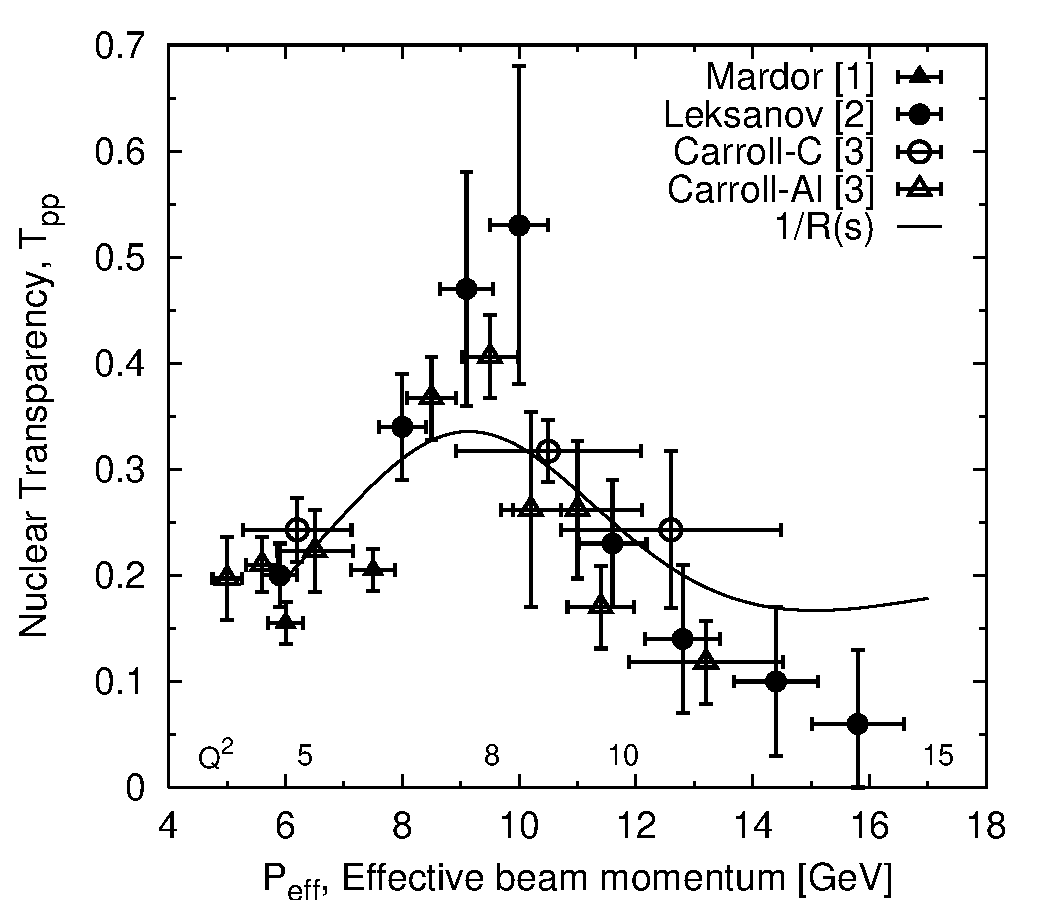
\includegraphics[width=0.6\textwidth]{chap2/ap2p.pdf}
    \caption{Transparency values $T_{pp}$ versus $p_{eff}$ for quasielastic
             proton scattering from carbon and aluminum (scaled by
             $(27/12)^{1/3}$) targets~\cite{Aclander_2004}.
             The solid curve is the inverse of $R(s)$ defined in
             equation~\ref{eqn:ap2p_rs}.
            }
    \label{fig:ap2p}
\end{figure}

\subsubsection{Interference between two terms}
One explanation focuses on interference between the amplitudes of two
perturbative QCD processes~\cite{Ralston_1988}, resulting in a transparency
that oscillates with $s$.
In this model, the effect of the energy-dependent phase shift on the scattering
amplitude can be respresented by
\begin{equation}
    M = M_{QC} + e^{i\phi(s) + i \delta_1}\left|M_L\right|
\end{equation}

Here $\delta_1$ is an energy-independent phase shift and $\phi(s)$ has a known
energy dependence analogous to renormalization-group
evolution~\cite{Pire_1982, Ralston_1982, Sen_1983}
\begin{equation}
    \phi(s) \propto \ln \ln \left( \frac{s}{\Lambda_{QCD}^2} \right)
\end{equation}


The first term $M_{QC}$ is a hard amplitude dominant at high energies,
characterizing quarks separated by small transverse
distances~\cite{Brodsky_1973, Brodsky_1975, Matveev_1973, Lepage_1980};
so-called ``quark counting rules'' predict that the asymptotic energy
dependence of $pp$ scattering at a fixed angle $\theta_{cm}$ should look like
$\frac{d\sigma}{dt}\sim s^{-10}$.
The second term $M_L$ is the Landshoff mechanism---three-gluon exchange in the
t-channel~\cite{Landshoff_1974, Landshoff_1980}.
It is suppressed at high energies, but may be significant at intermediate
energies~\cite{Mueller_1981}.


Taking the ratio of the differential cross section $d\sigma/dt$ to the
quark-counting prediction $d\sigma_0/dt$
yields the following ratio, with parameters $\rho_1$ and $K$ to be determined
by a fit to data:
\begin{align} \label{eqn:ap2p_rs}
    R(s) &= \frac{d\sigma}{dt_{pp}} \bigg/ \frac{d\sigma_0}{dt_{pp}}
          = s^{10} \frac{d\sigma}{dt_{pp}} \\
         &\propto 1 + \rho_1 s^{1-K} \cos\left[\phi(s)+\delta_1\right] + \rho_1^2 s^{2-2k}/4
\end{align}

\begin{figure}[!h]
    \centering
    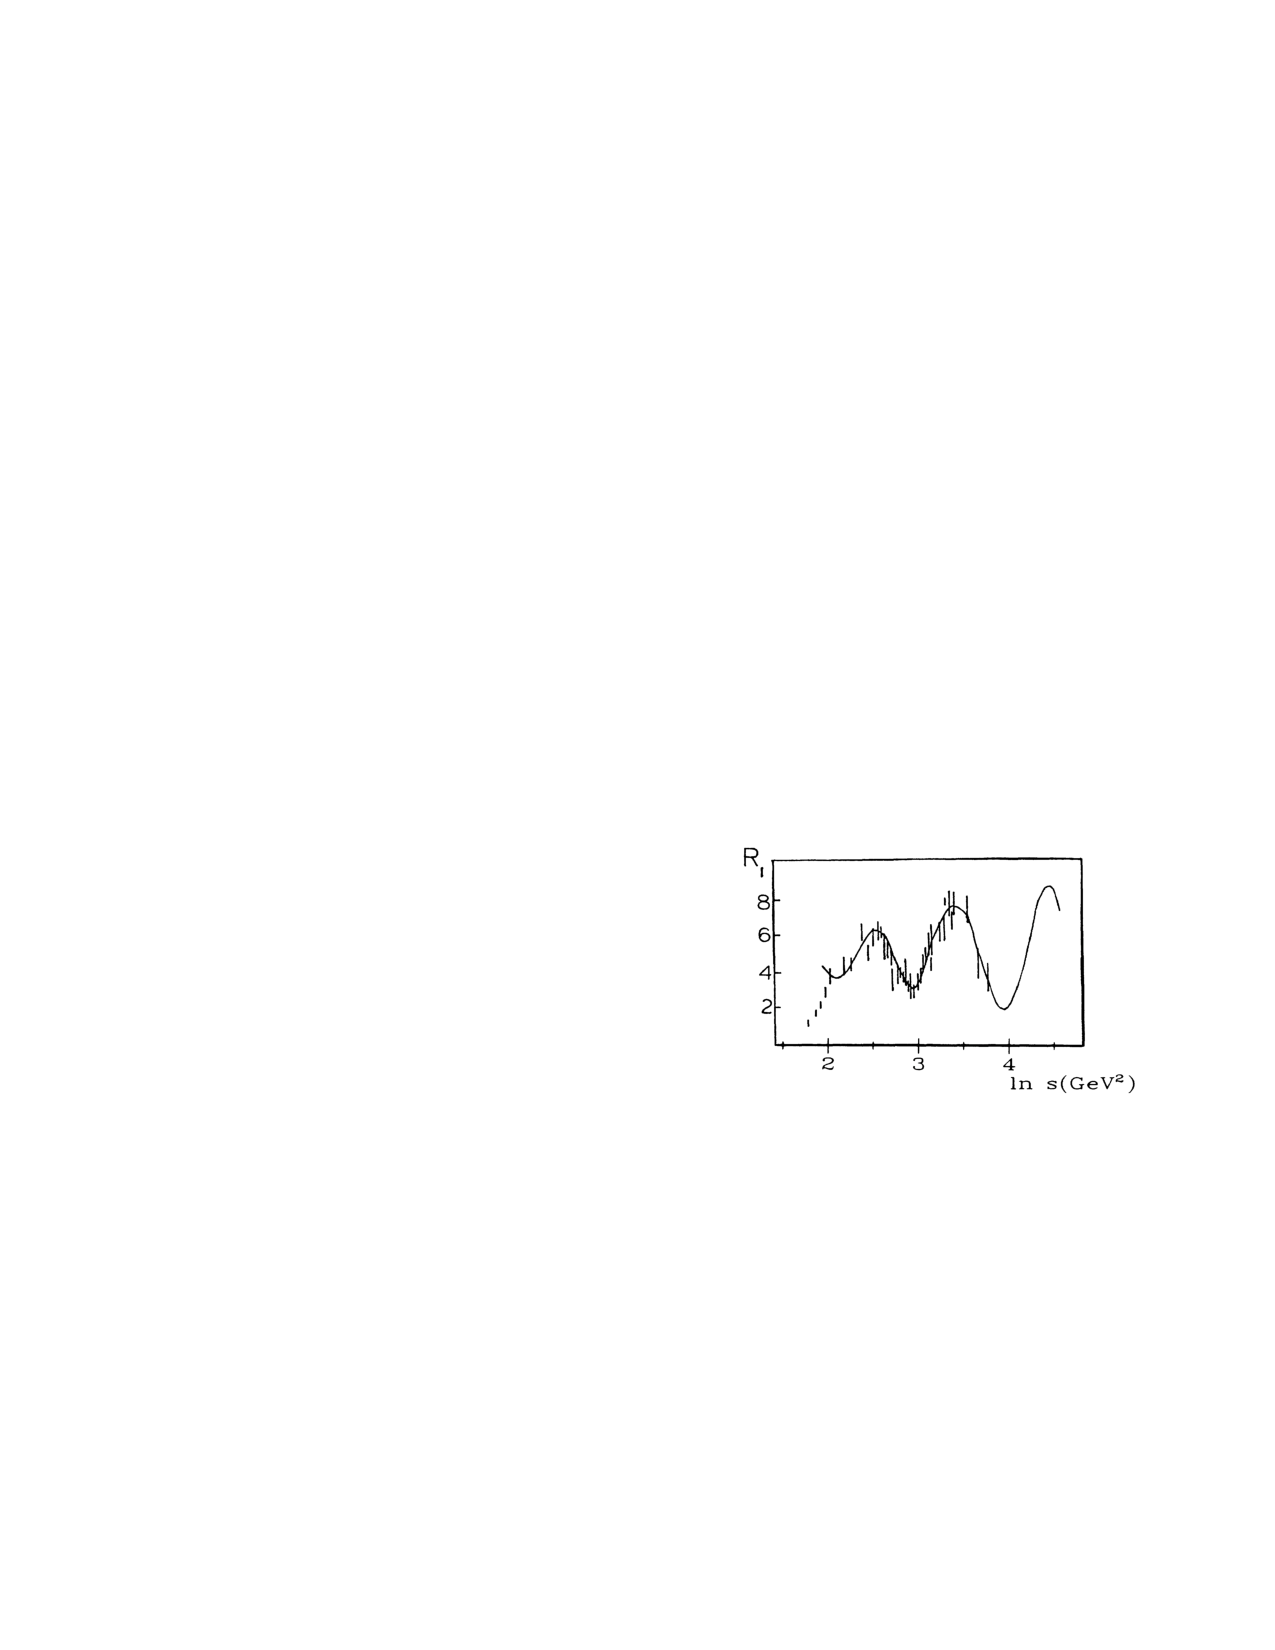
\includegraphics[width=0.6\textwidth]{chap2/pire_1982_R}
    \caption{A fit of $R(s)$, defined in equation~\ref{eqn:ap2p_rs}, to data taken from~\cite{Sivers_1976}
             for $pp$ elastic scattering at fixed angle
             $\theta_{cm}=\SI{90}{\deg}$.
             Figure reproduced from~\cite{Pire_1982}.
            }
    \label{fig:pire_1982_R}
\end{figure}

Similarly, this model predicts the energy dependence of the transparency $T$:
\begin{align}
    T(s) &= \frac{1}{A}\frac{d\sigma\left(pA \rightarrow pp(A-1)\right)/dt}
                            {d\sigma\left(pp \rightarrow pp\right)/dt} \\
         &\propto \frac{1 + \rho_A s^{1-K} \cos\left[\phi(s)+\delta_A\right] + \rho_A^2 s^{2-2k}/4}
                       {1 + \rho_1 s^{1-K} \cos\left[\phi(s)+\delta_1\right] + \rho_1^2 s^{2-2k}/4}
\end{align}


For large A such that $\rho_As^{1-K}\ll1$, the numerator is independent of
energy and transparency is approximately $1/R(s)$.
Given the form of $R(s)$ in equation~$\ref{eqn:ap2p_rs}$, the transparency
should oscillate as a function of $s$, with another rise potentially
appearing around $s\approx\SI{20}{\giga\electronvolt}$.

\subsubsection{New physics?}
The second explanation is that the energy dependence corresponds to a resonance
or some threshold for new physics, such as a charm quark resonance or some
multi-quark state.

\subsection{Quasielastic electron scattering}

\subsection{Meson production}

\subsection{Pion electro/photo-production}

\subsection{$\rho^0$ meson electronproduction}
